\section{Performantie}
\label{sec:evaluatie-performantie}

%TODO eq (tim)
De bekomen data voor de vier raamwerken aan de hand van formule~\ref{eq:performantie-enhanced} wordt weergegeven in tabel \ref{tabel:evaluatie-performantie}.
Voor de score van performantie geldt hoe kleiner, hoe beter.
\begin{table}
\centering
\pgfplotstabletypeset[
  begin table=\begin{tabular}{p{8cm} p{0.8cm} p{0.8cm} p{0.8cm} p{0.8cm} p{0.3cm}},
  end table=\end{tabular},
  skip coltypes=true,
  col sep=comma,
  string type,
  header=true,
  columns={Performantie,ST,Kendo,jQM,Lungo},
  columns/Performantie/.style={column name=\textbf{Performantie}, column type={l}},
  columns/ST/.style={column name=\textbf{\sta}, column type={l}},  
  columns/jQM/.style={column name=\textbf{\jqma}, column type={l}},    
  columns/Kendo/.style={column name=\textbf{\kendoa}, column type={l}},   
  columns/Lungo/.style={column name=\textbf{\lungoa}, column type={l}}, 
  every head row/.style={
    before row=\toprule,
    after row=\midrule},
  every last row/.style={
  	before row=\midrule,
    after row=\bottomrule}
]{tabellen/performantie.csv}
\caption{Overzicht van performantie.}
\label{tabel:evaluatie-performantie}
\end{table}

Het is duidelijk dat op vlak van performantie \lungo{} het beste scoort, kort gevolgd door \jqm{} en \st{}.
Dit wordt verklaard doordat de eerste twee raamwerken geen ontwerppatroon afdwingen waardoor er ook een kleinere \js{}-code dient te worden gedownload ten opzichte van raamwerken die wel een ontwerppatroon afdwingen (zie ook tabel \ref{tabel:raamwerken-tabel}).
\kendo{} en \st{} komen respectievelijk op de voorlaatste en laatste plaats.
\st{} scoort het slechtst op gemiddelde downloadtijd, maar behaalt de beste score op gebruikerservaring.

Eerst zal in sectie~\ref{sec:evaluatie-downloadtijd} de gemiddelde downloadtijd gedetailleerd worden besproken.
Hieropvolgend zal in sectie~\ref{sec:evaluatie-gebruikerservaring} de gebruikerservaring worden besproken.
Als laatste wordt de performantie getoetst aan andere metrieken in sectie~\ref{sec:evaluatie-performantie-duiding}.


%%%%%%%%%%%%%%%%%%

\subsection{Gemiddelde downloadtijd}
\label{sec:evaluatie-downloadtijd}

%TODO gonzalo: beschrijven formules
De gemiddelde downloadtijd wordt bepaald volgens formule \ref{eq:totale-downloadtijd}.
De gemiddelde downloadtijd voor de loginapplicatie als de loginapplicatie uit cache worden bepaald volgens formule~\ref{eq:totale-downloadtijd} en \ref{eq:totale-gebruikerservaring}.
De uitkomsten hiervan worden weergegeven in tabel~\ref{tabel:evaluatie-performantie-downloadtijd}.
Om beter de spreiding van deze downloadtijd op de acht apparaten te kunnen bekijken, wordt op figuur \ref{fig:performantie-login-boxplot} de downloadtijd uitgezet in een boxplot.
Eerst zal deze van de loginapplicatie worden besproken en vervolgens van de loginapplicatie uit cache.

\begin{table}
\centering
\pgfplotstabletypeset[
  begin table=\begin{tabular}{p{8cm} p{0.8cm} p{0.8cm} p{0.8cm} p{0.8cm} p{0.3cm}},
  end table=\end{tabular},
  skip coltypes=true,
  col sep=comma,
  string type,
  header=true,
  columns={Performantie,ST,Kendo,jQM,Lungo},
  columns/Performantie/.style={column name=\textbf{Performantie}, column type={l}},
  columns/ST/.style={column name=\textbf{\sta}, column type={l}},  
  columns/jQM/.style={column name=\textbf{\jqma}, column type={l}},    
  columns/Kendo/.style={column name=\textbf{\kendoa}, column type={l}},   
  columns/Lungo/.style={column name=\textbf{\lungoa}, column type={l}}, 
  every head row/.style={
    before row=\toprule,
    after row=\midrule},
  every last row/.style={
  	before row=\midrule,
    after row=\bottomrule}
]{tabellen/performantie-downloadtijd.csv}
\caption{Gemiddelde downloadtijd van de loginapplicatie.}
\label{tabel:evaluatie-performantie-downloadtijd}
\end{table}

\begin{figure}
  \centering
  \subfloat[Loginapplicatie]{
    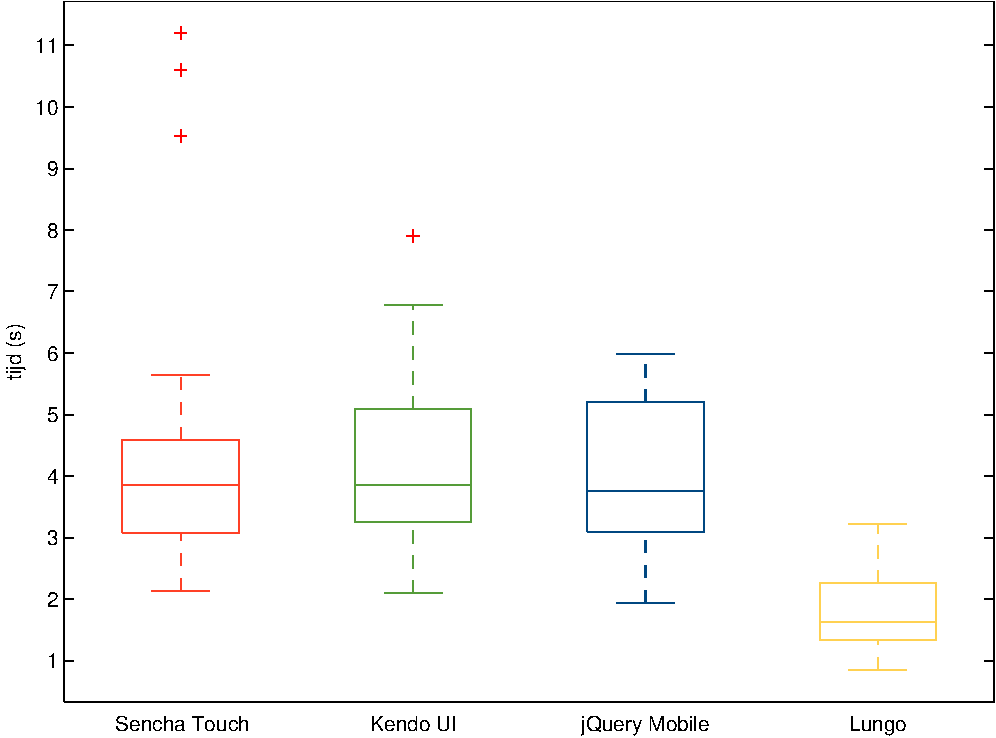
\includegraphics[width=0.85\textwidth]{figuren/performantie-login.pdf}
    \label{fig:performantie-login}
  }
  \quad
  \subfloat[Loginapplicatie uit cache]{
    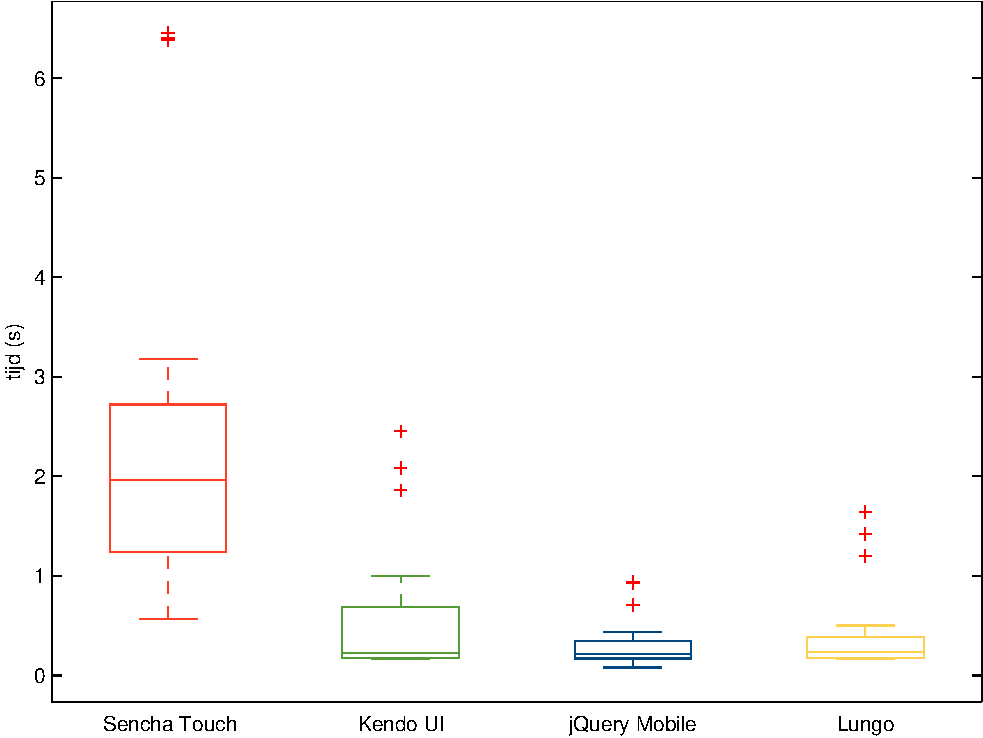
\includegraphics[width=0.85\textwidth]{figuren/performantie-login-cache.pdf}
    \label{fig:performantie-login-cache}
  }
  \caption{Downloadtijden van de loginapplicatie.}
  \label{fig:performantie-login-boxplot}
\end{figure}

\paragraph{Loginapplicatie}
\lungo{} behaalt de eerste plaats (zie figuur \ref{fig:performantie-login}).
\jqm{} en \kendo{} behalen respectievelijk een tweede en derde plaats.
\lungo{} is zelfs meer dan de helft sneller dan \jqm{}, \kendo{} of \st{}.
Deze drie raamwerken behalen quasi dezelfde downloadtijd.
\st{} behaalt de laatste plaats.
Dit wordt verklaard door het gebruik van een ontwerppatroon waardoor een grotere \js{}-code dient te worden gedownload ten opzichte van raamwerken die geen ontwerppatroon afdwingen (zie ook tabel \ref{tabel:raamwerken-tabel}).

\paragraph{Loginapplicatie uit cache}
Als naar de versie uit cache wordt gekeken, scoren \kendo{}, \jqm{} en \lungo{} hetzelfde (zie figuur \ref{fig:performantie-login-cache}).
Daarentegen behaalt \st{} telkens een veel tragere tijd.
Enerzijds komt dit doordat de drie eerstgenoemde raamwerken enkel gebruik maken van HTML5 Application Cache.
\st{} gebruikt daarnaast ook nog een eigen mechanisme waardoor de grotere downloadtijd wordt verklaard (zie \ref{app:performantie-st}).
Anderzijds gebruiken de drie eerstgenoemde raamwerken Yeoman om de applicatie te bouwen.
De webapplicaties gemaakt in \st{} gebruiken daarentegen Sencha Cmd.

%%%%%%%%%%%%%%%%%%

\subsection{Gebruikerservaring}
\label{sec:evaluatie-gebruikerservaring}
In tabel \ref{tabel:evaluatie-performantie-gebruikerservaring} wordt de totaalscore voor de gebruikerservaring getoond.

\begin{table}
\centering
\pgfplotstabletypeset[
  begin table=\begin{tabular}{p{8cm} p{0.8cm} p{0.8cm} p{0.8cm} p{0.8cm} p{0.3cm}},
  end table=\end{tabular},
  skip coltypes=true,
  col sep=comma,
  string type,
  header=true,
  columns={Apparaat,ST,Kendo,jQM,Lungo},
  columns/Apparaat/.style={column name=\textbf{Apparaat}, column type={l}},
  columns/ST/.style={column name=\textbf{\sta}, column type={l}},  
  columns/jQM/.style={column name=\textbf{\jqma}, column type={l}},    
  columns/Kendo/.style={column name=\textbf{\kendoa}, column type={l}},   
  columns/Lungo/.style={column name=\textbf{\lungoa}, column type={l}},   
  every head row/.style={
    before row=\toprule,
    after row=\midrule},
  every last row/.style={
  	before row=\midrule,
    after row=\bottomrule}
]{tabellen/performantie-gebruikerservaring.csv}
\caption{Gebruikerservaring van het scrollen door een lange lijst.}
\label{tabel:evaluatie-performantie-gebruikerservaring}
\end{table}

\st{} behaalt de maximale score.
Dit wil zeggen dat op alle toestellen het scrollen door de lijst van \st{} het vlotst ging.
\jqm{} werd zes keer als tweede beste beoordeeld. 
Op de \htc{} liep \kendo{} vlotter,  op de \ipadi{} was \lungo{} nummer twee.
De lijst genereren met \kendo{} op iOS-toestellen was onmogelijk omdat de applicatie de browser liet crashen.
De reden waarom alsook de grens van het aantal lijstelementen wanneer \kendo{} crasht op iOS-toestellen werd door tijdsbudget niet gecontroleerd.
Een mogelijke denkpiste is dat \kendo{} een overhead genereerd die het maximale toegelaten geheugen voor het iOS-besturingssysteem overschrijdt.
Op Android toestellen kon de \kendo{} lijst echter wel worden getoond.
De score van \kendo{} is dus slechts voor vier apparaten.

%%%%%%%%%%%%%%%%%%

\subsection{Duiding}
\label{sec:evaluatie-performantie-duiding}

In wat volgt zullen metrieken worden besproken die de score van de performantie zullen duiden.
De data van de metrieken is weergegeven in tabel~\ref{tabel:performantie-verklaring} en figuur \ref{fig:performantie}.
%TODO Gonzalo wat in tabel en figuur te zien?

\begin{table}
\centering
\pgfplotstabletypeset[
  begin table=\begin{tabular}{p{8cm} p{1cm} p{1cm} p{1cm} p{1cm}},
  end table=\end{tabular},
  skip coltypes=true,
  col sep=comma,
  string type,
  header=true,
  columns={Performantiemetrieken,jQM,ST,Kendo,Lungo},
  columns/Performantiemetrieken/.style={column name=\textbf{Performantie}, column type={l}},  
  columns/ST/.style={column name=\textbf{\sta}, column type={c}},
  columns/jQM/.style={column name=\textbf{\jqma}, column type={c}},
  columns/Kendo/.style={column name=\textbf{\kendoa}, column type={c}},
  columns/Lungo/.style={column name=\textbf{\lungoa}, column type={c}},
  every head row/.style={
    before row=\toprule,
    after row=\midrule},
  every last row/.style={
    after row=\bottomrule}
]{tabellen/performantie/performantie-verklaring.csv}
\caption{Duiding bij performantie van de loginapplicatie.}
\label{tabel:performantie-verklaring}
\end{table}


\begin{figure}
 \centering
 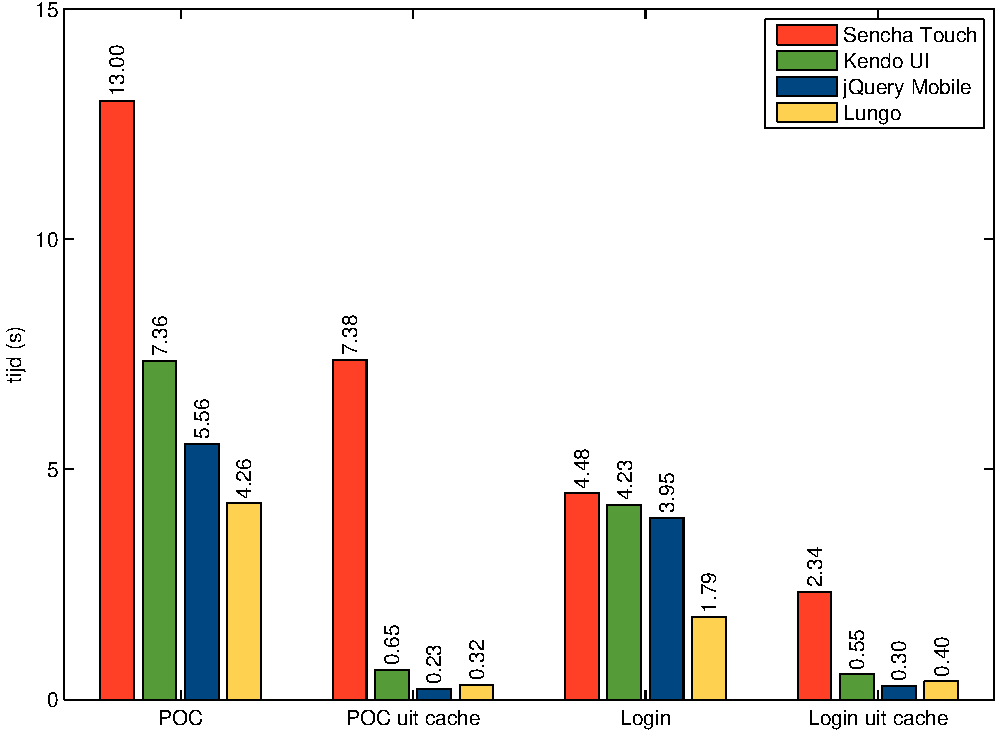
\includegraphics[width=\textwidth]{figuren/performance-nl.pdf}
 \caption{Gemiddelde downloadtijd van POC,  POC uit cache,  login en login uit cache voor elk raamwerk.}
 \label{fig:performantie}
\end{figure}


\paragraph{Downloadtijd POC versus loginapplicatie}
Op figuur \ref{fig:performantie} wordt de gemiddelde downloadtijd van de POC en login, zowel gewoon als uit cache, voor de vier raamwerken getoond.
Voor de gemiddelde downloadtijd per apparaat per raamwerk wordt verwezen naar appendix \ref{app:performantie}.

%%% De cache factor van ST is constant (gemiddeld 1,8)
%%% De andere raamwerken hebben een beduidend grotere cache factor 

De tragere downloadtijd van \st{},  zoals geconcludeerd door de downloadtijd van de login applicatie, wordt bevestigd.
Het verschil van downloadtijden voor de POC wordt nog uitvergroot.
Het mechanisme voor het updaten van de cache zal \st{} nog meer vertragen bij de POC.

Indien \st{} buiten beschouwing wordt gelaten, duurt de eerste keer laden van de POC gemiddeld $5,73\unit{s}$. 
Het laden van de versie uit cache duurt slechts gemiddeld $400\unit{ms}$.
De eerste keer laden van de loginapplicatie duurt gemiddeld $3,32\unit{s}$.
Indien deze uit cache komt, duurt dit gemiddeld nog slechts gemiddeld $420\unit{ms}$.


Indien enkel de downloadtijd in rekening wordt gebracht en \st{} buiten beschouwing wordt gelaten, kan er gezien worden dat de downloadtijden $< 10\unit{s}$.
Dit zijn aanvaardbare tijden volgens Jakob Nielsen~\cite{Nielsen1993}.
De gebruiker zal de vertraging waarnemen maar de aandacht niet verliezen.
Het initieel laden van de POC implementatie met \st{} moet van een laadscherm worden voorzien omdat de downloadtijd $> 10\unit{s}$.


\paragraph{Google Page Speed}
De score op 100 die Google Page Speed~\cite{Morgan2011} aan de applicatie toekent kan in tabel~\ref{tabel:performantie-verklaring} worden teruggevonden.
\st{} scoort het best ($96$),  gevolgd door \lungo{} ($82$),  \kendo{}($73$) en \jqm{}($71$).

Er kan geconcludeerd worden dat Sencha Cmd de applicatie optimaal weet te bouwen,  er is het minst plaats voor verbetering.
Hoewel \st{} de meeste tijd vraagt om te laden, zal het na het laden sneller werken.
Dit wordt bevestigd in de voorbije testen.

Alle implementaties worden aangeraden een tekenset te specificeren en gebruik te maken van het cachegeheugen van de browser.
Dit laatste is een suggestie om de maximale duur van documenten in de cache een week in de toekomst te zetten.
De huidige implementaties hebben een vervaldatum van slechts tien minuten.
Beide werkpunten hebben volgens Google Page Speed een lage prioriteit.
Alle raamwerken buiten \st{} worden aangeraden om de \js-code uitgesteld te parsen.
Bij \kendo{} en \jqm{} heeft dit werkpunt een hogere prioriteit in tegenstelling tot \lungo{}.
Dit komt omdat \lungo{} maar een kleiner aantal bytes moet verwerken.
De implementatie van \st{} wordt ook aangeraden om vraagtekens uit URLs te verwijderen.
Dit zou de oorzaak kunnen zijn voor het niet-cachen van bestanden.


\paragraph{Downloadgrootte}
De PCAP-bestanden die werden gebruikt om de downloadtijd op te meten bevatten ook de grootte van de pakketten die moeten worden opgehaald.
Omdat pakketten verloren gaan, zullen ontvangen bestanden incompleet zijn en moeten ze worden herverzonden.
Hierdoor zal het aantal ontvangen bytes variëren van meting tot meting.
De performantietesten werden op acht toestellen uitgevoerd en elke test werd drie keer uitgevoerd.
Het gemiddelde van alle downloadgroottes bepaalt de grootte zoals deze kan worden teruggevonden in tabel~\ref{tabel:performantie-verklaring}.
\kendo{} moest de meeste data ophalen ($296.50$~kB),  gevolgd door \st{} ($247.59$~kB), \jqm{} ($185.43$~kB) en \lungo{} ($59.75$~kB).
%Opmerkelijk is dat \lungo{} meer data moet ophalen maar toch een snellere downloadtijd behaald.
% Ook het verschil in downloadgrootte tussen de POC en loginapplicatie is opmerkelijk.
% Bij \jqm{} kan slechts een daling van $4.74\%$ worden waargenomen.
% \st{} en \lungo{} waren gelijkaardig en de downloadgrootte daalde respectievelijk met $78.02\%$ en $76.01\%$.
% De reductie in data bij \kendo{} was $45.30\%$.

% Bij alle applicaties werd de \js{}- en CSS-code verkleind en samengevoegd.
% De HTML-code werd niet gewijzigd.
% Tabel~\ref{tabel:performantie-verklaring} bevat het aantal lijnen HTML-code dat moest worden opgehaald.
%Hieruit is duidelijk te zien welke raamwerken opmaakgedreven zijn.